\documentclass[11pt]{article}

% Packages
\usepackage[czech]{babel}
\usepackage[utf8]{inputenc}
\usepackage[useregional]{datetime2}
\usepackage[T1]{fontenc}
\usepackage[a4paper, total={15.24cm, 23.32cm}]{geometry}
\usepackage[thinlines]{easytable}
\usepackage{graphicx}
\usepackage[ampersand]{easylist}
\usepackage{changepage}
\usepackage{float}
\usepackage{color}
\usepackage{enumitem}
\usepackage{hyperref}
\usepackage{minted}

% Config
\renewcommand{\baselinestretch}{1.2} 
\setitemize{itemsep=0pt}
\hypersetup{
	colorlinks,
	citecolor=black,
	filecolor=black,
	linkcolor=black,
	urlcolor=black
}
\title{\textbf{II. Softwarové inženýrství}}
\date{\small\vspace{-9ex}Update: \today}
\setminted{fontsize=\small,baselinestretch=1}

\begin{document}
\maketitle
\setcounter{tocdepth}{1}
\tableofcontents
\pagebreak

\section{Modelování databázových systémů, konceptuální modelování, datová analýza, funkční analýza; nástroje a modely.}
\subsection{Architektura mikroprocesorů}
\textbf{Architektura procesoru} je náčrt struktury a funkčnosti systému. Je charakterizována výčtem \textbf{registrů} a jejich funkcí, vnitřních a vnějších \textbf{sběrnic}, způsobem \textbf{adresování} a \textbf{instrukčním souborem}.

\textbf{Registr} je malé úložiště dat v mikroprocesoru s rychlým přístupem, které slouží jako \textbf{pracovní paměť} během výpočtů.

\textbf{Sběrnice} je soustava vodičů pro \textbf{přenos informací} mezi více účastníky na principu \uv{jeden vysílá, ostatní přijímájí.} Podle typu přenášené informace je dělíme na \textit{datové}, \textit{adresové} a \textit{řídící}. V praxi však díky multiplexu může jít o jedny dráty.

\subsection{Procesory CISC a RISC}
V dnešní době se ustálilo dělení počítačů do dvou základních kategorií podle typu používaného procesoru:
\begin{itemize}
	\item{\textbf{CISC} -- počítač se složitým souborem instrukcí (\textit{Complex Instruction Set Computer})}
	\item{\textbf{RISC} -- počítač s redukovaným souborem instrukcí (\textit{Reduced Instruction Set Computer})}
\end{itemize}

\subsubsection{CISC}
\begin{itemize}
	\item Procesory s \textbf{komplexním instrukčním souborem}.
	\item Instrukce mají \textbf{proměnlivou délku} i \textbf{dobu vykonání}.
	\item \textbf{Vysoká složitost instrukcí} $\,\to\,$ nutný systematický návrh řadiče procesoru.
	\item Vykonání strojové instrukce probíhá posloupností mikrooperací (předepsána mikroinstrukcí v řídící paměti).
	\item Procesor obsahuje relativně \textbf{nízký počet registrů}.
	\item Operace provedená i \textbf{složenou instrukcí} (např. násobení) může být \textbf{nahrazena} sledem jednodušších strojových instrukcí (\textit{sčítání a bitové posuny}) $\,\to\,$ mohou být ve výsledu vykonány rychleji, než hardwarově implementovaná složená varianta.
	\item {Označení \textbf{CISC} bylo zavedeno jako \textbf{protiklad} až poté, co se prosadily procesory RISC, které mají instruční sadu naopak maximálně redukovanou (pouze jednoduché operace, tj. žádné složené, jsou stejně dlouhé a jejich vykonání trvá stejnou dobu).}
	\item {Obvyklou chybou je domněnka, že procesory CISC mají více strojových instrukcí, než procesory RISC. Ve skutečnosti nejde o absolutní počet, ale o \textbf{počet různých druhů operací}, které procesor sám přímo umí vykonat na hardwarové úrovni (tj. již z výroby). Procesor CISC tak může například paradoxně obsahovat jen jednu strojovou instrukci pro danou operaci (např. \textit{logické operace}), zatímco procesor RISC může tuto operaci obsahovat jako několik strojových instrukcí, které stejnou operaci umí provést nad různými registry.}
\end{itemize}
\begin{figure}[H]
\centering
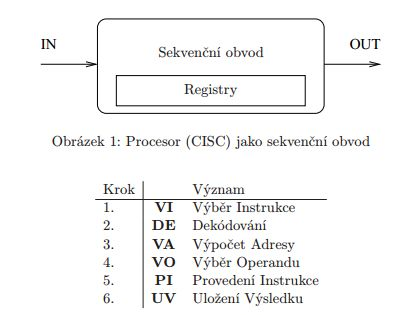
\includegraphics[width=0.6\textwidth]{assets/1_cisc_sekv}
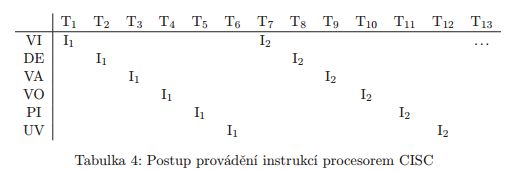
\includegraphics[width=0.6\textwidth]{assets/1_cisc_instrukce}
\end{figure}

\subsubsection{RISC}
\begin{itemize}
\item {\textbf{Počet instrukcí a způsobů adresování je malý, ale zůstává úplný}, aby bylo možno provést vše $\,\to\,$ v tomhle se liší od CISC}.
\item {Instrukce jsou vytvořeny pomocí obvodu $\,\to\,$ jednodušší na výrobu než CISC}.
\item Je menší počet instrukcí, takže složitější instrukce se nahradí větším počtem jednodušších.
\item To způsobuje nárust kódu. Zároveň ale vznikly rychlejší sběrnice, tj rychlejší proud dat do procesoru.
\item {Používá se \textbf{zřetězené zpracování instrukcí} (Blíže popsáno níže)}. 
\item {Instrukce se provádějí jen nad registry}.
\item {Navýšený počet registrů $\,\to\,$ delší program}.
\item {Instrukce mají \textbf{jednotný formát} -- délku i obsah}.
\item {Komunikace s pamětí pouze pomocí instrukcí \textbf{LOAD / STORE}, adresování i práce je celkově rychlejší}.
\item V návaznosti je využívaná cache pro co nejrychlejší přístup dat.
\item Využívá se \textbf{predikce skoků}, takže se začnou načítat data, která pravděpodobně budou v další instrukci potřeba.
\item {\textbf{Každý strojový cyklus znamená dokončení jedné instrukce}}.
\item {Řešení problémů s frontou instrukcí}.
\item {Mikroprogramový řadič může být nahrazen rychlejším obvodem}.
\item {Představitelé \textbf{ARM, MOTOROLA 6800, INTEL i960, MIPS R6000}}.
\end{itemize}
\begin{figure}[H]
\centering
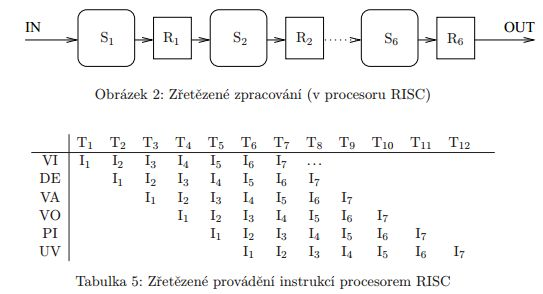
\includegraphics[width=0.6\textwidth]{assets/1_risc_zretezeni}
\end{figure}

\subsection{Von Neumannovo schéma počítače}

John Von Neumann definoval v roce \textbf{1945} základní koncepci počítače (EDVAC) \textbf{řízeného obsahem paměti}. Od té doby se objevilo několik odlišných modifikací, ale v podstatě se \textbf{počítače v dnešní době} konstruují podle tohoto modelu. Ve svém projektu si von Neumann stanovil určitá kritéria a principy, které musí počítač splňovat, aby byl použitelný univerzálně. Můžeme je ve stručnosti shrnout do následujících bodů:
\begin{itemize}
\item Počítač se skládá z paměti, řídící jednotky, aritmeticko--logické jednotky, vstupní a  výstupní jednotky.
\begin{enumerate}
\item \textbf{ALU} -- aritmeticko-logická jednotka (aritmetic-logic unit) => jednotka provádějící veškeré aritmetické výpočty a logické operace. Obsahuje sčítačky, násobičky a komparátory.
\item  \textbf{Operační paměť} -- slouží k uchování zpracovávaného programu, zpracovávaných dat a výsledků výpočtu.
\item \textbf{Řídící jednotka} -- řídí činnost všech částí počítače. Toto řízení je prováděno pomocí řídících signálů, které jsou zasílány jednotlivým modulům. Řadiči jsou pak zpět zasílané stavové hlášení. Dnes řadič spolu s ALU tvoří jednu součástku, a to procesor neboli CPU (Central Processing Unit).
\item \textbf{Vstup/Výstup} -- zařízení určené pro vstup dat, a výstup zpracovaných výsledků.
\end{enumerate}
\item Struktura pc je \textbf{nezávislá na typu řešené úlohy} (univerzálnost), \textbf{počítač se programuje obsahem paměti}.
\item Následující krok počítače je závislý na kroku předešlém.
\item \textbf{Instrukce} a \textbf{data} jsou v téže paměti.
\item Paměť je rozdělena do \textbf{paměťových buněk stejné velikosti (Byte)}, jejichž pořadová čísla se využívají jako adresy.
\item Program je tvořen posloupností instrukcí, které se vykonávají jednotlivě v pořadí, v jakém jsou zapsány do paměti.
\item Změna pořadí prováděných instrukcí se provádí \textbf{skokovými instrukcemi} (podmíněné nebo nepodmíněné skákání na adresy). 
\item Čísla, instrukce, adresy a znaky se značí v \textbf{binární soustavě}.
\end{itemize}
\begin{figure}[H]
\centering
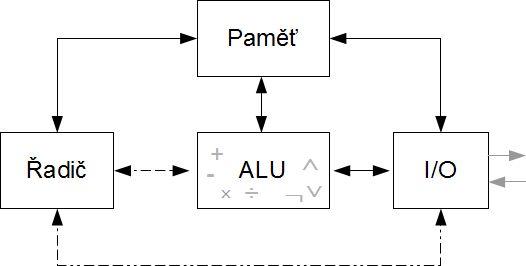
\includegraphics[width=0.6\textwidth]{assets/1_vonNeumann}
\end{figure}

\subsubsection{Nevýhody Von Neumannovy koncepce ve srovnání s dnešními PC}
\begin{itemize}
\item Podle von Neumannova schématu počítač pracuje \textbf{vždy nad jedním programem}. Toto vede k velmi špatnému využití strojového času. Dnes je obvyklé, že počítač \textbf{zpracovává paralelně více programů} zároveň - tzv. \textbf{multitasking}.
\item Počítač může mít i více jak jeden procesor.
\item Podle Von Neumanova schématu mohl počítač pracovat pouze v tzv. \textbf{diskrétním režimu}, kdy byl do paměti počítače zaveden program, data a pak probíhal výpočet. V průběhu výpočtu již nebylo možné s počítačem dále interaktivně komunikovat.
\item Dnes existují \textbf{vstupní/výstupní} zařízení, např. pevné disky a páskové mechaniky, které umožňují vstup i výstup.
\item Program se do paměti nemusí zavést celý, ale je možné zavést pouze jeho část a ostatní části zavádět až v případě potřeby.
\end{itemize}

\noindent\makebox[\textwidth]{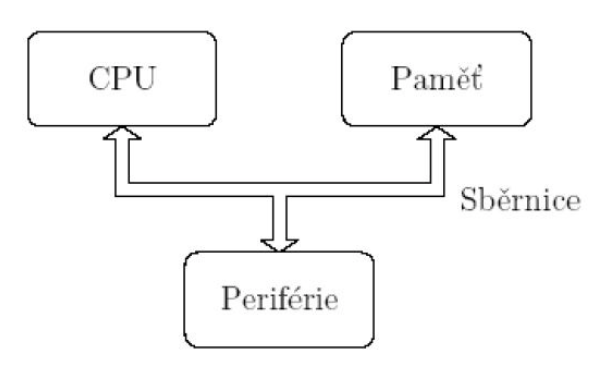
\includegraphics[width=8cm]{assets/1_neuman2}}

\subsubsection*{Výhody}
\begin{itemize}
	\item[$+$] \textbf{Rozdělení paměti} pro kód a data určuje programátor, řídící jednotka přistupuje pro  data i instrukce jednotným způsobem.
	\item[$+$] \textbf{Jedna sběrnice} ->  jednodušší levnější výroba.
\end{itemize}
\subsubsection*{Nevýhody}
\begin{itemize}
	\item[$-$] \textbf{Společné uložení dat a kódu} může mít za následek přepsání vlastního programu.
	
	\item[$-$] \textbf{Jedna sběrnice} je omezující.
\end{itemize}

\subsection{Hardvardské schéma počítače}
Několik let po von Neumannovi, přišel vývojový tým odborníků z Harvardské univerzity s vlastní koncepcí počítače, která se sice od Neumannovy příliš nelišila, ale odstraňovala některé její nedostatky. V podstatě jde pouze o \textbf{oddělení paměti pro data a program}. Abychom si mohli obě koncepce porovnat, můžeme vycházet ze zjednodušených schémat.
\newline

\noindent\makebox[\textwidth]{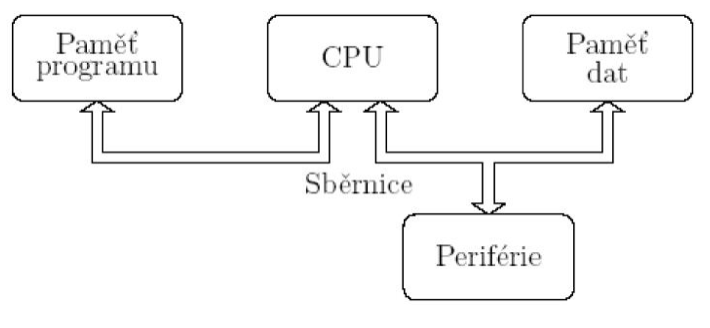
\includegraphics[width=8cm]{assets/1_harvard}}

\subsubsection*{Výhody}
\begin{itemize}
	\item[$+$]\textbf{Program se nepřepíše} (oddělené paměti pro data a program).
	\item[$+$]Dvě sběrnice umožňují \textbf{paralelní} načítání instrukcí a dat.
	\item[$+$]Paměti mohou být vyrobeny \textbf{odlišnými technologiemi }a každá může mít jinou nejmenší adresovací jednotku (8 bitů pro instrukce a 8, 16 nebo 32 pro data).
\end{itemize}


\subsubsection*{Nevýhody}
\begin{itemize}
\item[$-$]2 sběrnice mají \textbf{vyšší nároky na vývoj} řídící jednotky a jsou také dražší a složitější na výrobu.
\item[$-$]Paměť je \textbf{rozdělena} už od \textbf{výrobce}.
\item[$-$]Nevyužitou část dat \textbf{nelze využít }po program a obráceně.
\end{itemize}

\pagebreak
\subsection{Principy urychlování činnosti procesorů}
\begin{itemize}
	\item{Speciální kódování dle potřeby dané úlohy}.
	\item{Speciální výpočetní jednotky dle potřeby dané úlohy (FFT -- rychlá fourierova transformace)}.
	\item{Paralelní zpracování (násobné výpočetní jednotky)}.
	\item{\textbf{Zřetězové zpracování instrukcí} (pipelining)}.
	\item{Využití cache pamětí (L1, L2, L3)}.
	\item{Predikce skoků}
\end{itemize}
\subsubsection{Paralelní zpracování}
Zpracování více elementárních úloh běží součastně.
\begin{figure}[H]
\centering
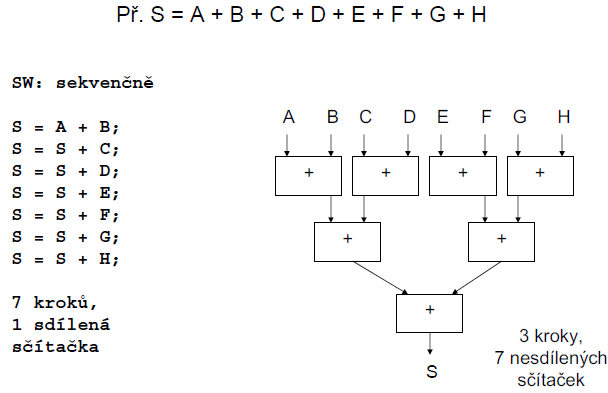
\includegraphics[width=0.6\textwidth]{assets/1_paralelni_zpracovani.png}
\end{figure}

\subsubsection{Zřetězené zpracování instrukcí (pipelining)}
Princip zřetězení se značně překrývá s principy procesorů RISC.
%\subsection{Problémy zřetězeného zpracování}
 Základní myšlenkou je \textbf{rozdělení zpracování jedné instrukce} mezi různé části procesoru a tím i dosažení možnosti \textbf{zpracovávat} \textbf{více instrukcí }najednou. Pro dosažení tohoto zřetězení je nutné rozdělit úlohu do posloupnosti dílčích úloh, z nichž každá může být vykonána \textbf{samostatně}, např. oddělit načítaní a ukládání dat z paměti od provádění výpočtu instrukce a tyto části pak mohou běžet souběžně. To znamená že musíme osamostatnit jednotlivé části sekvenčního obvodu tak, aby každému obvodu odpovídala jedna fáze zpracování instrukcí. Všechny fáze musí být \textbf{stejně časově náročné}, jinak je rychlost \textbf{degradována} na nejpomalejší z nich. Fáze zpracování je rozdělena minimálně na 2 úseky:
\begin{itemize}
\item \textbf{Načtení} a \textbf{dekódování} instrukce.
\item \textbf{Provedení} instrukce a případné uložení výsledku.
\end{itemize}
Zřetězení se stále vylepšuje a u novějších procesorů se již můžeme setkat stále s více řetězci rozpracovaných informací (více pipelines), dnes je standardem 5 pipelines.

\subsubsection{Problém a predikce skoků}
Největší problém spočívá v \textbf{plnění zřetězené jednotky}, hlavně při provádění \textbf{podmíněných skoků}, kdy během stejného počtu cyklů se vykoná více instrukcí. U pipelingu se instrukce následující po skoku vyzvedává dřív, než je skok dokončen. \textbf{Primitivní implementace} vyzvedává vždy \textbf{následující instrukci}, což vede k tomu, že se vždy mýlí, pokud je skok nepodmíněný. Pozdější implementace mají \textbf{jednotku předpovídání skoku (1bit)}, která vždy správně \textbf{předpoví nepodmíněný skok} a s použitím cache se záznamem předchozího chování programu se pokusí předpovědět i cíl podmíněných skoků nebo skoků s adresou v registru nebo paměť. V případě, že se predikce nepovede, bývá nutné vyprázdnit celou pipeline a začít vyzvedávat instrukce ze správné adresy, což znamená relativně \textbf{velké zdržení}. Související problémem je přerušení.

\subsubsection{Plnění fronty instrukcí}
Pokud se dokončí skoková instrukce, která odkazuje na jinou část kódu, musejí být instrukce za ní zahozeny (\textit{problém plnění fronty instrukcí}).
\begin{itemize}
	\item{U malého zřetězení \textbf{neřešíme}}.
	\item{Používání bublin na vyprázdnění pipeline, \textbf{naplněníní prázdnými instrukcemi}}.
	\item{\textbf{Predikce skoku} -- vyhrazen jeden bit předurčující, zda se skok provede či nikoliv}.
\end{itemize}
\begin{itemize}
	\item{\textbf{Statická} -- součást instrukce $\,\to\,$ řeší programátor nebo kompilátor}
	\item{\textbf{Dynamická} 
			\begin{itemize}
					\item{\textbf{jednobitová} -- zaznamenává jestli se skok provedl, či ne (1/ 0)}
					\item{\textbf{dvoubitová} -- metoda zpožděného skoku $\,\to\,$ v procesoru řeší se např. tabulkou s 4 kB instrukcí}
			\end{itemize}
		}
\end{itemize}
Zřetězené zpracování přináší urychlení výpočtu nejen v procesorech, ale i jiných číslicových obvodech (např. pro zpracování obrazu, bioinformatických dat apod.). Pokud použijeme zřetězené zpracování, musíme dodat řadu podpůrných obvodů a řešit řadu nových problémů. \textbf{Moderní procesory používají kromě zřetězení i další koncepty}:
\begin{itemize}
	\item{\textbf{Superskalární architektura} (zdvojení) -- když nastane podmíněný skok, začnou se vykonávat instrukce obou variant, nepotřebná část se pak zahodí. Tento způsob, pak vyžaduje vyřešit ukládání výsledku.}
	\item{\textbf{VLIW procesory} (Very long instruction word) -- umožňuje instrukční paralelismus (vykonávání několik nezávislých instrukcí souběžně), velmi dlouhé instrukční pakety}.
	\item{\textbf{Vektorové procesory} -- je navržený tak, aby dokázal vykonávat matematické operace nad celou množinou čísel v daném čase. Je opakem skalárního procesoru, který vykonává jednu operaci s jedním číslem v daném čase. }
	\item{\textbf{Vícevláknové procesory} }
\end{itemize}


\pagebreak
\section{Relační datový model, SQL; funkční závislosti, dekompozice a normální formy.}
\subsection{Specifikace požadavků}
Specifikace a analýza požadavků je první fáze vývoje softwaru. \textbf{Cílem je definovat požadavky na software a popsat jeho funkcionalitu}. Výsledkem této fáze by měly být dokumenty, které se stanou součásti smlouvy mezi zadavatelem a vývojovým týmem. \textbf{Kvalita} výsledného produktu je pak dána \textbf{mírou uspokojení požadavků zadavatele}.

V rámci specifikace požadavků je třeba analyzovat procesy u zadavatele, které bude software řešit, nebo s ním nějak jinak souvisí. K popisu těchto procesů dobře poslouží \textbf{Diagram případu užití}, \textbf{Sekvenční diagram} a \textbf{Diagram aktivit}.

\subsubsection{Cíle požadavků}
\begin{itemize}
\item chceme vytvořit a udržovat dohody se zákazníky a dalšími zainteresovanými stranami o tom, co by \textbf{systém měl dělat a proč},
\item aby vývojáři lépe pochopili \textbf{požadavky na systém},
\item definování \textbf{hranic systému},
\item vytvořit základ pro plánování \textbf{technického obsahu} interakcí,
\item poskytnout základ pro \textbf{odhad} \textbf{nákladů} a \textbf{času} na \textbf{vytvoření systému},
\item definovat \textbf{uživatelské rozhraní} pro systém, se zaměřením na potřeby uživatelů.
\end{itemize}

\subsubsection{Aktivity spojené s analýzou požadavků}
\begin{itemize}
	\item \textbf{Sběr požadavků} --  komunikace se zákazníky a uživateli za účelem získání jejich požadavků na systém.
	\item \textbf{Analýza požadavků} -- identifikování nejasných požadavků, nekompletních, nebo protichůdných a následné řešení těchto nesrovnalostí.
	\item \textbf{Zaznamenání požadavků} -- dokumentování požadavků v různých formách, jako běžný textový dokument, případy užití (use case), nebo specifikace procesů.
\end{itemize}
Požadavky je také nutno: \textbf{organizovat}, \textbf{dokumentovat}, \textbf{priorizovat}, \textbf{filtrovat} a \textbf{sledovat}.

\subsubsection{Typy požadavků -- FURPS}
\begin{itemize}
\item \textbf{Funkční požadavky (chování)} -- se používají k vyjádření chování systému zadáním jak vstupních tak i výstupních podmínek.
\item \textbf{Doplňující požadavky (nefunkční)}
\begin{itemize}
\item \textbf{Použitelnost (Usability)} -- se zabývá lidskými faktory, jako je vzhled, snadné používání, atd.
\item \textbf{Spolehlivost (Reliability)} --  četnost a závažnost selhání, obnovitelnost a přesnost.
\item \textbf{Výkon (Performance)} -- se zabývá množstvím transakcí, jako je rychlost, doba odezvy, atd.
\item \textbf{Podporovatelnost (Supportability)} -- řeší, jak těžké je udržet systém a další vlastnosti potřebné k udržení systému po jeho vydání.
\end{itemize}
\end{itemize}

\subsection{Diagram případů užití}
\textbf{Případ užití (use case)} -- je technika pro zdokumentování případného požadavku na nový systém, nebo změny na stávající systém. Každý use case poskytuje jeden nebo více scénářů, které zaznamenávají, jak by systém měl spolupracovat s koncovým uživatelem nebo jiným systémem.

Diagram případu užití popisuje \textbf{vztahy} mezi \textbf{aktéry} a jednotlivými \textbf{případy užití}. Součástí diagramu jsou:
\begin{itemize}
\item \textbf{Aktéři} -- definují \textbf{uživatele} či \textbf{jiné systémy}, kteří budou vstupovat do interakce s vyvíjeným softwarovým systémem.
\item \textbf{Relace (vztahy)} -- \textbf{vazby} a \textbf{vztahy} mezi aktéry a případy užití. V diagramu jsou znázorněny \textbf{šipkami případně čárami}.
\item \textbf{Případy užití} -- specifikující vzory chování  softwarovým systémem.  Každý případ užití lze chápat jako \textbf{posloupnost vzájemně navazujících transakcí} vykonaných \textbf{v dialogu mezi aktérem a vlastním softwarovým systémem}.
\item \textbf{Scénář} -- unikátní sekvence akcí skrz use-case (jedna cesta/instance provedení).
\end{itemize}
\textbf{Účelem} diagramu případů užití \textbf{je definovat co existuje vně vyvíjeného systému} (\textbf{aktéři}) a \textbf{co má být systémem prováděno (případy užití)}. Vstupem pro sestavení diagramu případů užití je \textbf{byznys model}, konkrétně modely podnikových procesů.  \textbf{Výsledkem} analýzy těchto procesů \textbf{je seznam požadovaných funkcí softwarového systému}, které podpoří nebo dokonce nahradí některé z uvedených aktivity jejich softwarovou implementací.

\begin{figure}[H]
	\centering
	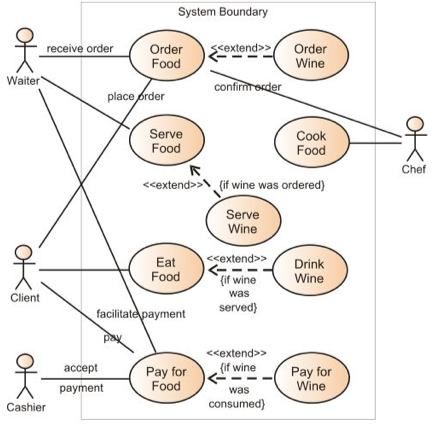
\includegraphics[width=0.7\textwidth]{assets/usecase.png}
\end{figure}

\noindent Pro složitější a obsáhlejší diagramy případů užití se zavadí \textbf{tři (+1) typy vztahů}:
\begin{itemize}
    \item \textbf{Relace} - bez typu (jen čára) značí přístup k UC, nejčastěji mezi aktéri a UC
\item \textbf{Include} – případ užití musí \textbf{obsahovat} jiný (UC s include se vždy provede před samotným UC).
\item \textbf{Extend} – případ užití může \textbf{rozšiřovat} jiný (UC s extend se může nebo nemusí provést).
\item \textbf{Generalizace} – případ užití může být \textbf{speciálním případem} jiného (dědičnost).
\end{itemize}

\subsubsection{Doporučená forma vytváření use-case}
\begin{itemize}
\item má vyjadřovat \textbf{co systém dělá} (ne jak) a co od něj očekávají aktéři,
\item měly by být používány jen pojmy problémové domény -- žádné neznámé termíny,
\item případy užití by měly být co \textbf{nejjednodušší}, ať jim rozumí i zadavatelé -- nepoužívat příliš \texttt{<include>} a \texttt{<extend>},
\item \textbf{nepoužívat} příliš funkční dekompozici (\textbf{specializaci}),
\item primární aktéři umístěni vlevo a pojmenováni krátkým podstatným jménem,
\item každý \textbf{aktér} by měl být \textbf{propojen s minimálně jedním use-case},
\item základní use case vlevo a další kreslit směrem doprava, rozšířující use-case směrem dolů.
\end{itemize}

\subsection{Sekvenční diagram}
Sekvenční diagram popisuje funkce systému z pohledu \textbf{objektů} a\textbf{ jejich interakcí}. Komunikace mezi objekty je \textbf{znázorněná v čase}, takže z diagramu můžeme vyčíst i životní cyklus objektu. 

Tento diagram popisuje jaké \textbf{zprávy} (\textbf{požadavky}) \textbf{jsou mezi objekty zasílány} \textbf{z pohledu času}. Diagram je tvořen \textbf{objekty uspořádanými do sloupců} a šipky mezi nimi odpovídají {vzájemně si zasílaným zprávám}. Zprávy mohou být {synchronní} nebo {asynchronní}. V případě \textbf{synchronních zpráv odesílatel čeká na odpověď} (odezvu) adresáta, v případě \textbf{asynchronní zprávy odesílatel nečeká} na odpověď a pokračuje ve vykonávání své činnosti. Souvislé provádění nějaké činnosti se v sekvenčním diagram vyjadřuje svisle orientovaným obdélníkem. Odezvu adresáta lze opět modelovat, v tomto případě tzv. \textbf{návratovou zprávou (přerušovaná čára)}. Tok času probíhá ve směru od shora dolů.
\\\\
\noindent\makebox[\textwidth]{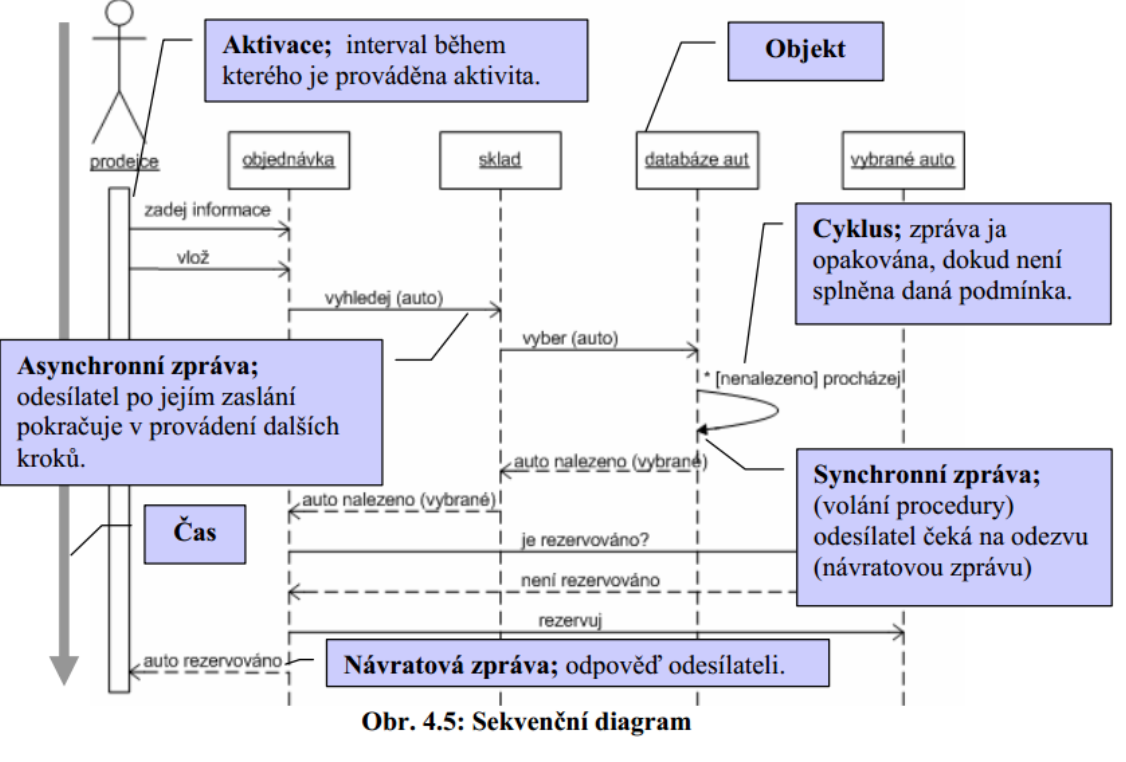
\includegraphics[width=1\textwidth]{assets/sekv}}

\pagebreak
\subsection{Diagram aktivit}
Diagram aktivit popisuje jednotlivé procesy pomocí aktivit reprezentující jeho (akční) \textbf{stavy} a \textbf{přechody mezi nimi}. Pokud aktivita "přetéká" v jednotlivých stavech mezi uživateli, mohou být tyto stavy naznačeny pomocí tzv \textbf{swimlines}.
\begin{figure}[H]
    \centering
    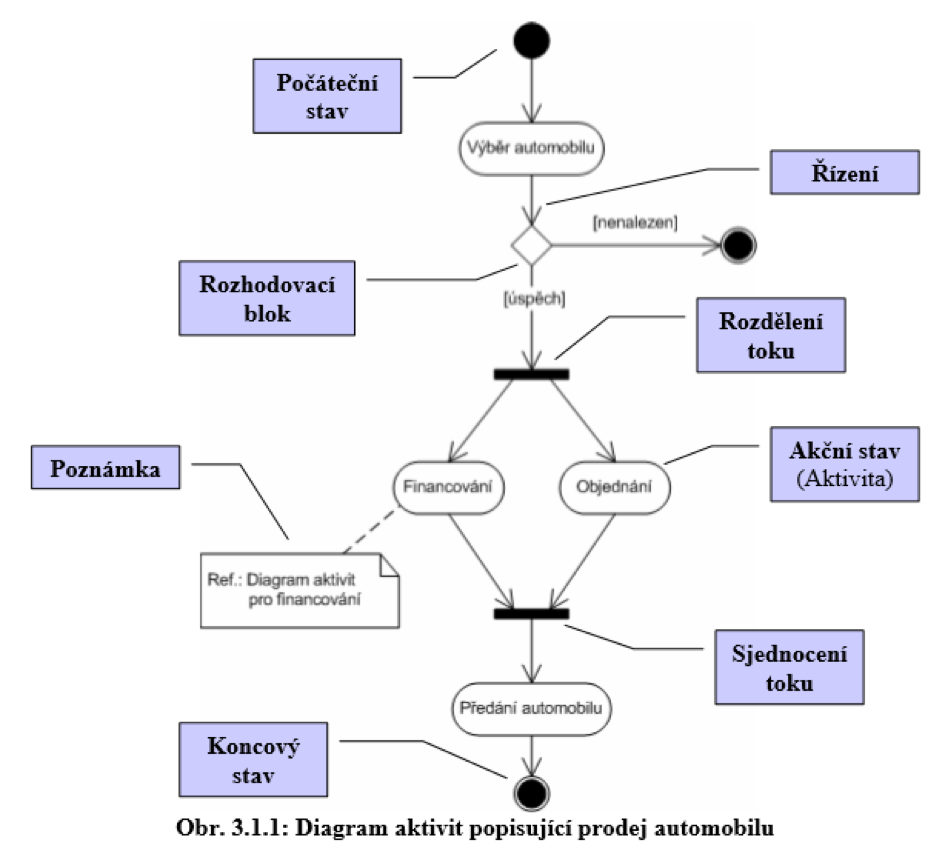
\includegraphics[width=1\textwidth]{assets/diag_aktivit.png}
\end{figure}

\begin{figure}[H]
	\centering
	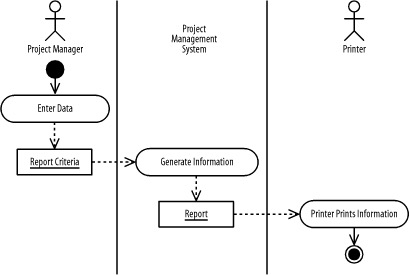
\includegraphics[width=1\textwidth]{assets/diag_aktivit_swimlines.gif}
\end{figure}

\pagebreak
\section{Transakce, zotavení, log, ACID, operace COMMIT a ROLLBACK; problémy souběhu, řízení souběhu: zamykání, úroveň izolace v SQL.}

\pagebreak
\section{Procedurální rozšíření SQL, PL/SQL, T-SQL, triggery, funkce, procedury, kurzory, hromadné operace.}

\pagebreak
\section{Základní fyzická implementace databázových systémů: tabulky a indexy; plán vykonávání dotazů.}

\pagebreak
\section{Objektově‐relační datový model a XML datový model: principy, dotazovací jazyky.}

\pagebreak
\section{Datová vrstva informačního systému; existující API, rámce a implementace, bezpečnost; objektově-relační mapování.}

\pagebreak
\section{Distribuované SŘBD, fragmentace a replikace.}

\end{document}
